% Custom TOC formatting with indentation and CGEL blue numbers
\titlecontents{section}
  [3cm]                                     % left margin (3cm indentation)
  {\addvspace{3pt}}                        % above code (reduced from default)
  {\sffamily\small\color{cgelblue}\thecontentslabel\quad}  % numbered entry format (sans, small, blue)
  {\sffamily\small}                        % numberless entry format (sans, small)
  {\rmfamily\scriptsize\color{cgelblue}\contentspage}  % filler and page (serif, small, blue page numbers)
  [\addvspace{1pt}]                        % below code (reduced spacing)

\setcounter{page}{43}
\thispagestyle{empty}
\chapternumber{2}
\grammartitle{Syntactic overview}
\grammarauthor{Rodney Huddleston}

\vspace{1cm}

\begin{spacing}{0.1}
\tableofcontents
\end{spacing}
\normalsize\color{black}

\newpage

\vspace*{3cm}
\noindent
Given the length and nature of this book, there will be relatively few readers who begin at the beginning and work their way through the chapters in order to the end. We envisage, rather, that readers will typically be reading individual chapters, or parts thereof, without having read all that precedes, and the main purpose of this syntactic overview is to enable the separate chapters to be read in the context of the grammar as a whole.

We begin by clarifying the relation between sentence and clause, and then introduce the distinction between canonical and non-canonical clauses, which plays an important role in the organisation of the grammar. The following sections then survey very briefly the fifteen chapters that deal with syntax (as opposed to morphology or punctuation), noting especially features of our analysis that depart from traditional grammar.

\cgelsection{Sentence and clause}
Syntax is concerned with the way words combine to form sentences. The sentence is the largest unit of syntax, while the word is the smallest. The structure of composite words is also a matter of grammar (of morphology rather than syntax), but the study of the relations between sentences within a larger text or discourse falls outside the domain of grammar. Such relations are different in kind from those that obtain within a sentence, and are outside the scope of this book.

We take sentences, like words, to be units which occur sequentially in texts, but are not in general contained one within another. Compare:

\begin{examples}
    \item \label{ex:1}
    \begin{examples}
        \item \label{ex:1i} Jill seems quite friendly.
        \item \label{ex:1ii} I think Jill seems quite friendly.
        \item \label{ex:1iii} Jill seems quite friendly, but her husband is extremely shy.
    \end{examples}
\end{examples}
{\addfontfeatures{LetterSpace=2.0}\textit{Jill seems quite friendly} is a sentence in [\ref{ex:1i}], but not in [\ref{ex:1ii}--\ref{ex:1iii}], where it is merely part of a sentence - just as in all three examples \textit{friend} is part of a word, but not itself a word.}

{\addfontfeatures{LetterSpace=-2.5}In all three examples \textit{Jill seems quite friendly} is a {clause}. This is the term we apply to a syntactic construction consisting (in the central cases) of a subject and a predicate. In} [\ref{ex:1ii}] one clause is contained, or \textit{embedded}, within a larger one, for we likewise have a subject-predicate relation between \textit{I} and \textit{think Jill seems quite friendly}. In [\ref{ex:1iii}] we have one clause \textit{coordinated} with another rather than embedded within it: \textit{her husband} is subject, \textit{is extremely shy} predicate and \textit{but} is the marker of the coordination relation. {\addfontfeatures{LetterSpace=-2.0}We will say, then, that in [\ref{ex:1i}--\ref{ex:1ii}] the sentence has the form of a clause, while in [\ref{ex:1iii}] it has the}


\newpage
\noindent form of a coordination of clauses (or a `clause-coordination').\footnote{Traditional grammar classifies the sentences in [\ref{ex:1}] as respectively \textit{simple}, \textit{complex}, and \textit{compound}, but this scheme conflates two separate dimensions: the presence or absence of embedding, and the presence or absence of coordination. Note that in \textit{I think Jill seems quite friendly, but her husband is extremely shy} there is both embedding and coordination. We can distinguish [\ref{ex:1i}--\ref{ex:1ii}] from [\ref{ex:1iii}] as \textit{non-compound} (or \textit{clausal}) vs \textit{compound}; [\ref{ex:1i}--\ref{ex:1ii}] could then be distinguished as \textit{simple} vs \textit{complex clauses} but no great significance attaches to this latter distinction, and we shall not make further use of these terms.} Within this framework, the clause is a more basic unit than the sentence.

To say that sentence [\ref{ex:1}\ref{ex:1i}] \textbf{has the form} of a clause is not to say that it consists of a clause, as the term `consists of' is used in constituent structure analysis of the type introduced in Ch.~1, §4.2. There is no basis for postulating any singulary branching here, with the clause functioning as head of the sentence. This is why our tree diagram for the example \textit{A bird hit the car} had the topmost unit labelled `clause', not `sentence.' `Sentence' is not a syntactic category term comparable to `clause, `noun phrase', `verb phrase', etc., and does not figure in our constituent structure representations.

Most work in formal grammar makes the opposite choice and uses \textit{sentence} (abbreviated S) rather than \textit{clause} in constituent structure representations. There are two reasons why we do not follow this practice. In the first place, it creates problems for the treatment of coordination. In [\ref{ex:1iii}], for example, not only the whole coordination but also the two clauses (\textit{Jill seems quite friendly} and \textit{but her husband is extremely shy}) would be assigned to the category \textit{sentence}. The coordination, however, is quite different in its structure from that of the clauses: the latter are subject-predicate constructions, while the coordination clearly is not. Most importantly, assigning the whole coordination to the same category as its coordinate parts does not work in those cases where there is coordination of different categories, as in:

\begin{examples}
    \item \label{ex:2} \itshape You must find out \ob the cost and whether you can pay by credit card\cb.
\end{examples}
Here the first coordinate, \textit{the cost}, is an NP while the second is, on the analysis under consideration, a sentence, but the whole cannot belong to either of these categories. We argue, therefore, that coordinative constructions need to be assigned to different categories than their coordinate parts. Thus we will say, for example, that \textit{Jill seems quite friendly} is a clause, while [\ref{ex:1iii}] is a clause-coordination, \textit{Jill and her husband} an \textit{NP-coordination}, and the bracketed part of [\ref{ex:2}] an NP/clause-coordination (a coordination of an NP and a clause).

The second reason why we prefer not to use `sentence' as the term for the syntactic category that appears in constituent structure representations is that it involves an unnecessary conflict with the ordinary, non-technical sense of the term (as reflected, for example, in dictionary definitions). Consider:

\begin{examples}\item
\noindent\begin{minipage}[t]{0.6\linewidth}
    a. \itshape The knife \uline{I used} was extremely sharp.
\end{minipage}\vspace{-\medskipamount}
\begin{minipage}[t]{0.4\linewidth}
    b. \itshape I'm keen \uline{for it to be sold}.
\end{minipage}\vspace{-\medskipamount}
\end{examples}
The underlined sequences are not sentences in the familiar sense of the term that we adopted above, according to which sentences are units of a certain kind which occur in succession in a text. The underlined expressions nevertheless contain a subject (\textit{I}, \textit{it}) and a predicate (\textit{used} and \textit{to be sold}), and hence belong in the same syntactic category as expressions like \textit{Jill seems quite friendly}. If we call this category `sentence' rather than `clause', the term `sentence' will have two quite different senses.



\cgelsection{Canonical and non-canonical clauses}
There is a vast range of possible clause constructions, and if we tried to make descriptive statements covering them all at once, just about everything we said would have to be heavily qualified to allow for numerous exceptions. We can provide a simpler, more orderly description if in the first instance we confine our attention to a set of basic, or canonical, constructions, and then describe the rest derivatively, i.e. in terms of how they differ from the canonical constructions. 

The contrast between canonical and non-canonical clauses is illustrated in the following examples:

\begin{examples}\small
\item \label{ex:4}
\noindent\begin{minipage}[t]{0.5\linewidth}
\centering\textsc{canonical}\par\vspace{\smallskipamount}
    \begin{examples}
        \item \label{ex:4i}
            \textnormal{a.} Kim referred to the report.
        \item \label{ex:4ii}
            \textnormal{a.} She was still working.
        \item \label{ex:4iii}
            \textnormal{a.} Pat solved the problem.
        \item \label{ex:4iv}
            \textnormal{a.} Liz was ill.
        \item \label{ex:4v}
            \textnormal{a.} He has forgotten the appointment.
    \end{examples}
\end{minipage}\vspace{-\medskipamount}%
\hspace{2em}%
\begin{minipage}[t]{0.4\linewidth}
{\centering\textsc{non-canonical}\par}\vspace{\smallskipamount}
    b. \itshape Kim did not refer to the report.
    
    \textnormal{b.} Was she still working?
    
    \textnormal{b.}~The problem was solved by Pat.
    
    \textnormal{b.} He said \uline{that Liz was ill}.
    
    \textnormal{b.} Either he has overslept \uline{or he has forgotten the appointment}.
\end{minipage}
\end{examples}
\medskip
\cgelsubsection{Dimensions of contrast between canonical and non-canonical constructions}

\noindent
The examples in [\ref{ex:4}] illustrate five major dimensions of contrast between canonical and non-canonical clauses. In each case the canonical clause is syntactically more basic or elementary than the non-canonical one.

The examples in [\ref{ex:4}\ref{ex:4ii}] differ in {polarity}, with [a] positive and [b] negative. In this example, the negative differs from the positive not just by virtue of the negative marker \textit{not} but also by the addition of the semantically empty auxiliary \textit{\textbf{do}}.

The contrast in [\ref{ex:4}\ref{ex:4ii}] is one of {clause type}, with [a] declarative and [b] interrogative. The syntactic difference in this particular pair concerns the relative order of subject and predicator: in [a] the subject occupies its basic or default position before the predicator, while in [b] the order is inverted. In the pair \textit{She finished the work} and \textit{Did she finish the work?} the interrogative differs from the declarative both in the order of elements and in the addition of the auxiliary \textit{\textbf{do}}. All canonical clauses are declarative; non-canonical clauses on this dimension also include exclamatives (\textit{What a shambles it was!}) and imperatives (\textit{Sit down}).

In [\ref{ex:4}\ref{ex:4iii}], canonical [a] is {active} while [b] is {passive}. These clauses differ strikingly in their syntactic form, but their meanings are very similar: there is a sense in which they represent different ways of saying the same thing. More precisely, they have the same propositional content, but differ in the way the information is presented - or `packaged'. The passive is one of a number of non-canonical constructions on this dimension. Others include preposing (e.g. \textit{Most of them we rejected}, contrasting with canonical \textit{We rejected most of them}), the existential construction (e.g. \textit{There were several doctors on board}, contrasting with \textit{Several doctors were on board}), and the it-cleft (e.g. \textit{It was Pat who spoke first}, contrasting with \textit{Pat spoke first}).

The underlined clause in [\ref{ex:4}\ref{ex:4iv}b] is {subordinate}, whereas [a] is a {main clause}. In this example, the non-canonical clause is distinguished simply by the presence of the subordinator \textit{that}, but many kinds of subordinate clause differ from main clauses more


\newpage

\noindent radically, as for example in \textit{This tool is very easy to use}, where the subordinate clause consists of just the VP subordinator \textit{to} together with the predicator, with both subject and object left unexpressed. The clause in which a subordinate clause is embedded is called the \textbf{matrix clause} -- in [\ref{ex:4iv}b], for example, subordinate \textit{that Liz was ill} is embedded within the matrix clause \textit{He said that Liz was ill}. Subordination is {recursive}, i.e. repeatable, so that one matrix clause may be embedded within a larger one, as in \textit{I think he said that Liz was ill}.
\begin{itemize}
    \item Finally, the underlined clause in [\ref{ex:4v}b] is {coordinate}, in contrast to non-coordinate [\ref{ex:4v}]; it is marked as such by the coordinator \textit{or}. A greater departure from canonical structure is seen in \textit{Jill works in Paris, and her husband in Bonn}, where the predicator \textit{works} is missing.
\end{itemize}
It is of course possible for non-canonical constructions to combine, as in:
\begin{examples}
    \item \label{ex:5} \itshape I can't understand \uline{why I have not been questioned by the police}.
\end{examples}

The underlined clause here is negative, interrogative, passive, and subordinate. But these are independent properties, and we can describe the structure in terms of its difference from canonical clause structure on four separate dimensions.

\cgelsubsection{Counterparts}
In the examples of [\ref{ex:4}] we presented the non-canonical clauses side by side with their canonical \textbf{counterparts}, i.e. canonical clauses differing from them simply as positive rather than negative, declarative rather than interrogative, and so on. Where a clause combines two non-canonical features, its counterpart with respect to each feature will be non-canonical by virtue of retaining the other. Thus \textit{It wasn't written by Sue} has as its active counterpart \textit{Sue didn't write it} (non-canonical by virtue of being negative) and as its positive counterpart \textit{It was written by Sue} (non-canonical by virtue of being passive).

It must be emphasised, however, that not all non-canonical clauses have grammatically well-formed counterparts. Compare, for example:
\begin{examples}
\item \label{ex:6}
\noindent\begin{minipage}[t]{0.5\linewidth}
    \begin{examples}[nosep]\vspace{-6pt}
        \item \label{ex:6i}
            \textnormal{a.} I can't stay any longer.
        \item \label{ex:6ii}
            \textnormal{a.} Have they finished yet?
        \item \label{ex:6iii}
            \textnormal{a.} Kim was said to be the culprit.
        \item \label{ex:6iv}
            \textnormal{a.} There was an accident.
        \item \label{ex:6v}
            \textnormal{a.} If it hadn't been for you,\\ I couldn't have managed.
    \end{examples}
\end{minipage}\vspace{-\medskipamount}%
\begin{minipage}[t]{0.5\linewidth}
    b. \ungram \itshape I can stay any longer.
    
    \textnormal{b.} \ungram They have finished yet.
    
    \textnormal{b.} \ungram Said Kim to be the culprit.
    
    \textnormal{b.} \ungram An accident was.
    
    \textnormal{b.} \ungram It had been for you.
\end{minipage}\vspace{-\medskipamount}
\end{examples}
\medskip
Example [\ref{ex:6i}a] has no counterpart differing from it as positive vs negative, and similarly there is no declarative counterpart to interrogative [\ref{ex:6ii}a]. There is no active counterpart to the passive [\ref{ex:6iii}b], partly because \textit{\textbf{say}} + infinitival (with this sense) is restricted to the passive construction, partly -- and more generally -- because there is no element corresponding to the subject of an active clause. Existential [\ref{ex:6iv}a] differs from the one cited above (\textit{There were several doctors on board}) in that again there is no non-existential counterpart. And finally [\ref{ex:6v}a] contains a subordinate clause with no main clause counterpart. \textit{It had been for you} is of course grammatical in the interpretation where it refers to something identifiable in the context (cf. \textit{The parcel had been for you}), but that is not an interpretation of how it is used in [\ref{ex:6v}a].



\cgelsubsection{Syntactic processes}
We follow the practice of much traditional and modern grammar in commonly describing non-canonical structures in terms of syntactic processes. We talk, for example, of subject-auxiliary inversion, of passivisation and relativisation, or preposing and postposing, and so on. It should be made clear, however, that such process terminology is merely a convenient descriptive device. When we say, for example, that \textit{Is she still working?} involves subject-auxiliary inversion, we are not suggesting that a speaker actually starts with the declarative \textit{She is still working} and then reverses the order of the first two elements. Apart from the inherent implausibility of such an interpretation of process terminology, it cannot be reconciled with the point illustrated in [\ref{ex:6}], namely that in many cases a non-canonical clause has no grammatically well-formed canonical counterpart.\footnote{Note also that what we present in this book is an informal descriptive grammar, not a formal generative one: we are not deriving the `surface structure' of sentences from abstract `underlying structures.' Thus our process terminology is not to be interpreted as referring to operations performed as part of any such derivation.} It is always possible to translate the process description into an equivalent one couched in purely static terms. In the present example, we are merely saying that the order of the auxiliary and the subject is the opposite of that found in canonical clauses.

\cgelsubsection{Extension of the apparatus for the representation of syntactic structure}
The kind of syntactic analysis and representation we introduced in Ch.~1, §4.2, works well for canonical constructions, but needs some extension to cater for certain kinds of non-canonical construction. Compare, for example:

\begin{examples}
\item \label{ex:7}
\noindent\begin{minipage}[t]{0.5\linewidth}
    \begin{examples}\vspace{-6pt}
        \item \label{ex:7a}
            \textnormal{a.} Liz bought a watch.
    \end{examples}
\end{minipage}\vspace{-\medskipamount}%
\begin{minipage}[t]{0.5\linewidth}
    b. I wonder \uline{what Liz bought}.
\end{minipage}\vspace{-\medskipamount}
\end{examples}
While [a] is a canonical clause, the underlined clause in [b] is non-canonical in two respects: it is interrogative and subordinate. It is the interrogative feature that distinguishes it from the canonical [a], inasmuch as \textit{what} is understood as object of \textit{bought} although its position relative to the verb differs from that of the object \textit{a watch} in canonical [a]. (Clause [a] is not the declarative counterpart of \textit{what Liz bought} because it contains the NP \textit{a watch}, but it illustrates a comparable declarative structure.) The representations we propose are as in [\ref{ex:8}].

\begin{examples}
\item\label{ex:8}
\begin{forest}
where n children=0{% for each terminal node
    font=\itshape, 			% italics
    tier=word          			% align at the ``word" tier (bottom)
  }{
    l sep=1mm,
    inner sep=0mm,
  },
[Clause, name=top_a
    [\Subj{NP}
        [\Head{N}
            [Liz]
        ]
    ]
    [\Node{Predicate}{VP}
        [\Node{Predicator}{V}
            [bought]
        ]
        [\Obj{NP}
            [\Det{D}
                [a]
            ]
            [\Head{N}
                [watch]
            ]
        ]
    ]
]
\node at (top_a.west) [left=5mm] {a.};
\end{forest}
\hspace{2cm}
\begin{forest}
where n children=0{% for each terminal node
    font=\itshape, 			% italics
    tier=word          			% align at the ``word" tier (bottom)
  }{
    l sep=1mm,
    inner sep=0mm,
  },
[Clause, name=top_b
    [\Node{Prenucleus}{NP\textsubscript{i}}
        [\Head{N}
            [what]
        ]
    ]
    [\Node{Nucleus}{Clause}
        [\Subj{NP}
            [\Head{N}
                [Liz]
            ]
        ]
        [\Node{Predicate}{VP}
            [\Node{Predicator}{V}
                [bought]
            ]
            [\Node{Object}{GAP\textsubscript{i}}
                [---]
            ]
        ]
    ]
]
\node at (top_b.west) [left=5mm] {b.};
\end{forest}
\end{examples}

\noindent Structure [a] needs no commentary at this stage: it is of the type introduced in Ch.~1. In [b] \textit{what} precedes the subject in what we call the \textbf{prenucleus} position: it is followed~by

\newpage

\noindent the \textbf{nucleus}, which is realised by a clause with the familiar subject-predicate structure. Within this nuclear clause there is no overt object present. But the prenuclear \textit{what} is understood as object, and this excludes the possibility of inserting a (direct) object after \textit{bought}: *\textit{I wonder what Liz bought a watch}. We represent this by having the object realised by a \textbf{gap}, an abstract element that is \textbf{co-indexed} with \textit{what} (i.e. annotated~with the same subscript index, here `\textit{i}'): this device indicates that while \textit{what} is in prenuclear position, it also functions in a secondary or derivative sense as object of \textit{bought}.

Note that it would not be satisfactory to replace the `prenucleus' label by `object,' and then simply dispense with the object element on the right of \textit{bought}. Functions, we have said, are relational concepts and `object' is a relation between an NP and a VP construction. Directly labelling \textit{what} as object would not show that it is object of the VP headed by \textit{bought}. This can be seen more easily by considering such an example as [\ref{ex:9}], where the bracketed clause has the structure shown in [\ref{ex:10}]:

\begin{examples}
    \item \label{ex:9} \itshape I can't remember \ob what Max said Liz bought \_\cb.
\end{examples}

\begin{examples}
\item\label{ex:10}
\begin{forest}
where n children=0{% for each terminal node
    font=\itshape, 			% italics
    tier=word          			% align at the ``word" tier (bottom)
  }{
    l sep=2mm,
    s sep=10mm,
    inner sep=0mm,
  },
[Clause, name=top_10
    [\Node{Prenucleus}{NP\textsubscript{i}}
        [\Head{N}
            [what]
        ]
    ]
    [\Node{Nucleus}{Clause}
        [\Subj{NP}
            [\Head{N}
                [Max]
            ]
        ]
        [\Node{Predicate}{VP}
            [\Node{Predicator}{V}
                [said]
            ]
            [\Node{Comp}{Clause}
                [\Subj{NP}
                    [\Head{N}
                        [Liz]
                    ]
                ]
                [\Node{Predicate}{VP}
                    [\Node{Predicator}{V}
                        [bought]
                    ]
                    [\Node{Object}{GAP\textsubscript{i}}
                        [---]
                    ]
                ]
            ]
        ]
    ]
]
\end{forest}
\end{examples}

\noindent \textit{What} is in prenuclear position in the clause whose ultimate head is the verb \textit{said}, but it is understood as object of \textit{bought}, not \textit{said}. Simply labelling \textit{what} as object would not bring this out, whereas the co-indexed gap device does serve to relate \textit{what} to the \textit{bought} VP whose object it is.

We make use of the same device to handle subject-auxiliary inversion. Compare the structures in [\ref{ex:11}] for canonical \textit{He is ill} and interrogative \textit{Is he ill?} The nucleus in [b] is identical to structure [a] except for the gap, and this accounts for the fact that the functional relations between \textit{he, is,} and \textit{ill} are the same in the two clauses: \textit{he} is subject, \textit{ill} is predicative complement, and \textit{is} in [b] is shown to be predicator by virtue of its link to the gap element that fills the predicator position directly. Main clause interrogatives like \textit{What had Liz bought?} will thus have one prenucleus + nucleus construction (\textit{had} + \textit{Liz bought}) functioning as nucleus within another (\textit{what} + \textit{had Liz bought}).


\begin{examples}
\item\label{ex:11}
\begin{forest}
where n children=0{% for each terminal node
    font=\itshape, 			% italics
    tier=word          			% align at the ``word" tier (bottom)
  }{
    l sep=1mm,
    inner sep=0mm,
  },
[Clause, name=top_a
    [\Subj{NP}
        [\Head{N}
            [he]
        ]
    ]
    [\Node{Predicate}{VP}
        [\Node{Predicator}{V}
            [is]
        ]
        [\Node{PredComp}{AdjP}
            [ill]
        ]
    ]
]
\node at (top_a.west) [left=5mm] {a.};
\end{forest}
\hspace{2cm}
\begin{forest}
where n children=0{% for each terminal node
    font=\itshape, 			% italics
    tier=word          			% align at the ``word" tier (bottom)
  }{
    l sep=1mm,
    inner sep=0mm,
  },
[Clause, name=top_b
    [\Node{Prenucleus}{V\textsubscript{i}}
        [is]
    ]
    [\Node{Nucleus}{Clause}
        [\Subj{NP}
            [\Head{N}
                [he]
            ]
        ]
        [\Node{Predicate}{VP}
            [\Node{Predicator}{GAP\textsubscript{i}}
                [---]
            ]
            [\Node{PredComp}{AdjP}
                [ill]
            ]
        ]
    ]
]
\node at (top_b.west) [left=5mm] {b.};
\end{forest}
\end{examples}

\cgelsubsection{Organisation of the grammar}
The distinction between canonical and non-canonical clauses plays a major role in the organisation of the present grammar. The early chapters deal predominantly with the structure of canonical clauses, and with units smaller than the clause: phrases headed by nouns, adjectives, adverbs, and prepositions. Chs. 9-16 then focus on non-canonical constructions; subordination requires more extensive treatment than the other dimensions mentioned above, and is covered in Chs. 11-14. The final chapter devoted to syntax (Ch.~17) deals with deixis and anaphora, phenomena which cut across the primary part-of-speech distinction between nouns, verbs, etc. There follow two chapters dealing with the major branches of morphology, and we end with a short account of punctuation.


\cgelsection{The verb}
The head of a clause (the predicate) is realised by a VP, and the head of a VP (the predicator) is realised by a verb. The verb thus functions as the ultimate head of a clause, and is the syntactically most important element within it: properties of the verb determine what other kinds of element are required or permitted.\footnote{Since the verb is the ultimate head, we can identify clauses by the verb. In [\ref{ex:9}] of §2, for example, we can refer to the most deeply embedded clause as the \textit{buy} clause.}

\cgelsubsection{Inflection}
Most verbs have six inflectional forms, illustrated here for the lexeme \textit{\textbf{take}}:

\begin{examples}
\item \label{ex:12}
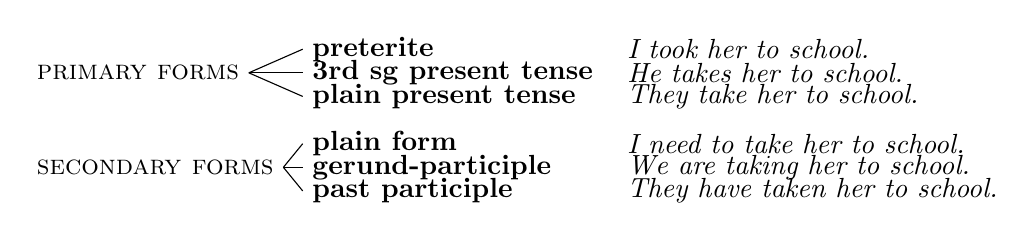
\begin{tikzpicture}[baseline=2.5mm]
% Primary forms
\node[anchor=west] (pf) at (0,0) {\textsc{primary forms}};
\node[anchor=west] (pret) at (3.5,0.3) {\textbf{preterite}};
\node[anchor=west] (3sg) at (3.5,0) {\textbf{3rd sg present tense}};
\node[anchor=west] (plain) at (3.5,-0.3) {\textbf{plain present tense}};
% Examples for primary forms
\node[anchor=west] at (7.5,0.3) {\textit{I took her to school.}};
\node[anchor=west] at (7.5,0) {\textit{He takes her to school.}};
\node[anchor=west] at (7.5,-0.3) {\textit{They take her to school.}};
% Draw diagonal lines for primary forms
\draw (pf.east) -- (pret.west);
\draw (pf.east) -- (3sg.west);
\draw (pf.east) -- (plain.west);
% Secondary forms
\node[anchor=west] (sf) at (0,-1.2) {\textsc{secondary forms}};
\node[anchor=west] (plainf) at (3.5,-0.9) {\textbf{plain form}};
\node[anchor=west] (gerund) at (3.5,-1.2) {\textbf{gerund-participle}};
\node[anchor=west] (pastp) at (3.5,-1.5) {\textbf{past participle}};
% Examples for secondary forms
\node[anchor=west] at (7.5,-0.9) {\textit{I need to take her to school.}};
\node[anchor=west] at (7.5,-1.2) {\textit{We are taking her to school.}};
\node[anchor=west] at (7.5,-1.5) {\textit{They have taken her to school.}};
% Draw diagonal lines for secondary forms
\draw (sf.east) -- (plainf.west);
\draw (sf.east) -- (gerund.west);
\draw (sf.east) -- (pastp.west);
\end{tikzpicture}
\end{examples}

\noindent Auxiliary verbs also have negative forms (\textit{She isn't here, I can't help it}, etc.), while the verb \textit{\textbf{be}} has two preterite forms (\textit{was} and \textit{were}) and three present tense forms (\textit{am, is, are}). The \textit{were} of \textit{I wish she were here} we take to be an irrealis mood form, a relic of an older system now found only with the verb \textit{\textbf{be}} with a 1st or 3rd person singular subject.

\newpage

The plain form occurs in three main constructions, one of which has two subtypes:

% Set a width for the first level of descriptions (IMPERATIVE, SUBJUNCTIVE)
\newlength{\labwidthA}
\settowidth{\labwidthA}{\textsc{subjunctive}\quad}
% Set a separate width for the descriptions inside item iii
\newlength{\labwidthB}
\settowidth{\labwidthB}{\textsc{bare infinitival}:\quad}
\begin{examples}
\item \label{ex:13}
    \begin{examples}
        % Items i and ii use the first width for alignment
        \item \label{ex:13i} \hspace{1.7em} \makebox[\labwidthA][l]{\textsc{imperative}} \hspace{2.2em}\itshape Take great care!
        \item \label{ex:13ii} \hspace{1.7em}  \makebox[\labwidthA][l]{\textsc{subjunctive}} \hspace{2.2em}\itshape It is essential \ob that he take great care\cb.
        % Item iii is now just a container for the next level
        \item \label{ex:13iii}
            \begin{examples}
                % The nested items a. and b. use the second width for their own alignment
                \item \label{ex:13iiia} \makebox[\labwidthB][l]{\textsc{\textit{to}-infinitival}:} \itshape I advise you \ob to take great care\cb.
                \item \label{ex:13iiib} \makebox[\labwidthB][l]{\textsc{bare infinitival}:} \itshape You must \ob take great care\cb.
            \end{examples}
    \end{examples}
\end{examples}

\noindent Note, then, that on our account imperative, subjunctive, and infinitival are clause constructions, not inflectional forms of the verb. \textit{To} in [\ref{ex:13iii}] is a VP subordinator, not part of the verb.

\cgelsubsection{Finite and non-finite}
These terms likewise apply to clauses (and by extension VPs), not to verb inflection. Finite clauses have as head a primary form of a verb or else a plain form used in either the imperative or the subjunctive constructions. Non-finite clauses have as head a gerund-participle or past participle form of a verb, or else a plain form used in the infinitival construction.

\cgelsubsection{Auxiliary verbs}
Auxiliary verbs are distinguished syntactically from other verbs (i.e. from lexical verbs) by their behaviour in a number of constructions, including those illustrated in:
\begin{examples}
\item \label{ex:14}
\noindent\begin{minipage}[t]{0.5\linewidth}
\centering{\textsc{auxiliary verb}}\par\vspace{\smallskipamount}
    \begin{examples}
        \item \label{ex:14i}
            \textnormal{a.} I have not seen them.
        \item \label{ex:14ii}
            \textnormal{a.} Will you go with them?
    \end{examples}
\end{minipage}\vspace{-\medskipamount}%
\begin{minipage}[t]{0.5\linewidth}
{\centering{\textsc{lexical verbs}}\par\vspace{\smallskipamount}}
    b. \ungram \itshape I saw not them.
    
    \textnormal{b.} \ungram Want you to go with them?
\end{minipage}
\end{examples}

\noindent Thus auxiliary verbs can be negated by a following \textit{not} and can invert with the subject to form interrogatives, but lexical verbs cannot. To correct [\ref{ex:14i}b/\ref{ex:14ii}b] we need to insert the dummy (semantically empty) auxiliary \textit{\textbf{do}}: \textit{I did not see them} and \textit{Do you want to go with them?} It follows from our syntactic definition that \textit{\textbf{be}} is an auxiliary verb not only in examples like \textit{She is working} or \textit{He was killed} but also in its copula use, as in \textit{They are cheap} (cf. \textit{They are not cheap} and \textit{Are they cheap?}).

Our analysis of auxiliary verbs departs radically from traditional grammar in that we take them to be heads, not dependents. Thus in \textit{She is writing a novel}, for example, \textit{is} is a head with \textit{writing a novel} as its complement; the constituent structure is like that of \textit{She began writing a novel}. Note, then, that \textit{is writing} here is not a constituent: \textit{is} is head of one clause and \textit{writing} is head of a non-finite subordinate clause.

\cgelsubsection{Tense and time}
There are two tense systems in English. The primary one is marked by verb inflection and contrasts {preterite} (\textit{She was ill}) and {present} (\textit{She is ill}). The secondary one is marked by the presence or absence of auxiliary \textit{have} and contrasts {perfect} (\textit{She is believed to have been ill}) and {non-perfect} (\textit{She is believed to be ill}). The perfect can combine with primary tense to yield compound tenses, {preterite perfect} (\textit{She had been ill}) and {present perfect} (\textit{She has been ill}).

{\addfontfeatures{LetterSpace=-2.0}
We distinguish sharply between the grammatical category of {tense} and the semantic category of {time}. In \textit{It started yesterday}, \textit{You said it started tomorrow}, and \textit{I wish it started tomorrow}}, for example, \textit{started} is a preterite verb-form in all three cases, but only in the

\newpage

\noindent first does it locate the starting in past time. Once this distinction is clearly drawn, it is easy to see that English has no future tense: \textit{will} and \textit{shall} belong grammatically with \textit{must, may,} and \textit{can}, and are modal auxiliaries, not tense auxiliaries.

\cgelsubsection{Aspect and aspectuality}
We make a corresponding distinction between grammatical {aspect} and semantic {aspectuality}. English has an aspect system marked by the presence or absence of the auxiliary \textit{\textbf{be}} contrasting {progressive} (\textit{She was writing a novel}) and {non-progressive} (\textit{She wrote a novel}). The major aspectuality contrast is between {perfective} and {imperfective}. With perfective aspectuality the situation described in a clause is presented in its totality, as a whole, viewed, as it were, from the outside. With imperfective aspectuality the situation is not presented in its totality, but viewed from within, with focus on the internal temporal structure or on some subinterval of time within the whole. The main use of progressive VPs is to express a particular subtype of imperfective aspectuality.

\cgelsubsection{Mood and modality}
Again, {mood} is a matter of grammatical form, {modality} a matter of meaning. Irrealis \textit{were}, mentioned above, is a residual mood-form, but the main markers of mood in English are the modal auxiliaries \textbf{\textit{can}}, \textbf{\textit{may}}, \textbf{\textit{must}}, \textbf{\textit{will}}, \textbf{\textit{shall}}, together with a few less central ones. 

Three main kinds of modal meaning are distinguished:
\newlength{\labwidthModal}
\settowidth{\labwidthModal}{\textsc{epistemic}\quad}
\begin{examples}
\item \label{ex:15}
    \begin{examples}
        \item \label{ex:15i}\makebox[\labwidthModal][l]{\textsc{deontic}} \textit{You must come in immediately.} \quad \textit{You can have one more turn.}
        \item \label{ex:15ii}\makebox[\labwidthModal][l]{\textsc{epistemic}} \textit{It must have been a mistake.} \quad \textit{You may be right.}
        \item\label{ex:15iii} \makebox[\labwidthModal][l]{\textsc{dynamic}} \textit{Liz can drive better than you.} \quad \textit{I asked Ed to go but he won't.}
    \end{examples}
\end{examples}
Deontic modality typically has to do with such notions as obligation and permission, or -- in combination with negation -- prohibition (cf. \textit{You can't have any more}). In the central cases, epistemic modality qualifies the speaker's commitment to the truth of the modalised proposition. While \textit{It was a mistake} represents an unqualified assertion, \textit{It must have been a mistake} suggests that I am drawing a conclusion from evidence rather than asserting something of whose truth I have direct knowledge. And \textit{You may be right} merely acknowledges the possibility that ``You are right" is true. Dynamic modality generally concerns the properties and dispositions of persons, etc., referred to in the clause, especially by the subject. Thus in [\ref{ex:15iii}] we are concerned with Liz's driving ability and Ed's willingness to go.

All three kinds of modality are commonly expressed by other means than by modal auxiliaries: lexical verbs (\textit{You don't need to tell me}), adjectives (\textit{You are likely to be fined}), adverbs (\textit{Perhaps you are right}), nouns (\textit{You have my permission to leave early}).


\cgelsection{The clause: complements}
Dependents of the verb in clause structure are either complements or modifiers. Complements are related more closely to the verb than modifiers. The presence or absence~of {\addfontfeatures{LetterSpace=-2.5}particular kinds of complement depends on the subclass of verb that heads the clause: the verb \textit{use}, for example, requires an object (in canonical clauses),} while \textit{arrive} excludes one.

\newpage\fontsize{9pt}{12pt}\selectfont
\noindent Moreover, the semantic role associated with an NP in complement function depends on the meaning of the verb: in \textit{He murdered his son-in-law}, for example, the object has the role of patient (or undergoer of the action), while in \textit{He heard her voice} it has the role of stimulus (for some sensation). Ch.~4 is mainly concerned with complements in clause structure.

\cgelsubsection{Subject and object}
\noindent One type of complement that is clearly distinguished, syntactically, from others is the {subject}: this is an external complement in that it is located outside the VP. It is an obligatory element in all canonical clauses. The {object}, by contrast, is an internal complement and, as just noted, is permitted -- or \textbf{licensed} -- by some verbs but not by others. Some verbs license two objects, indirect and direct. This gives the three major clause constructions:

\begin{examples}
\item \label{ex:16}
    \begin{tabular}{@{}lll@{}}
        \textsc{intransitive} & \textsc{monotransitive} & \textsc{ditransitive} \\
        a. \textit{She smiled} & b. \textit{He washed the car} & c. \textit{They gave me the key} \\
        \hspace{1.5em} S\hspace{1.3em}P & \hspace{1.5em} S\hspace{1.2em}P\hspace{2.6em}O\textsuperscript{d} & \hspace{1.7em} S\hspace{1.6em}P\hspace{1.6em}O\textsuperscript{i}\hspace{0.8em}O\textsuperscript{d}
    \end{tabular}
\end{examples}
The terms intransitive, monotransitive, and ditransitive can be applied either to the clause or to the head verb. Most verbs, however, can occur with more than one `complementation'. \textit{Read}, for example, is intransitive in \textit{She read for a while}, monotransitive in \textit{She read the newspaper}, and ditransitive in \textit{She read us a story}. 

Example [\ref{ex:16}c] has the same propositional meaning as \textit{They gave the key to me}, but \textit{to me} is not an indirect object, not an object at all: it is syntactically quite different from \textit{me} in [\ref{ex:16}c]. Objects normally have the form of NPs; \textit{to me} here is a complement with the form of a PP.

\cgelsubsection{Predicative complements}
A different kind of internal complement is the predicative (PC):
\begin{examples}
\item \label{ex:17}
    \begin{tabular}{@{}ll@{}}
        \textsc{complex-intransitive} & \textsc{complex-transitive} \\
        a. \textit{This seems a good idea }/\textit{ fair.} & b. \textit{I consider this a good idea }/\textit{ fair.} \\
        \hspace{1.5em}S\hspace{2em}P\hspace{4em}PC & \hspace{1.5em}S\hspace{1.2em}P\hspace{2.2em}O\textsuperscript{d}\hspace{3.2em}PC
    \end{tabular}
\end{examples}
{\addfontfeatures{LetterSpace=-2.5}We use the term {\textbf{complex-intransitive}} for a clause containing a predicative complement but no object, and {\textbf{complex-transitive}} for one containing both types of complement.}

The major syntactic difference between a predicative complement and an object is that the former can be realised by an adjective, such as \textit{fair} in these examples. Semantically, an object characteristically refers to some participant in the situation but with a different semantic role from the subject, whereas a predicative complement characteristically denotes a property that is ascribed to the referent of the subject (in a complex-intransitive) or object (in a complex-transitive).

\cgelsubsubsection{Ascriptive and specifying uses of the verb \textit{\textbf{be}}}
Much the most common verb in complex-intransitive clauses is \textit{\textbf{be}}, but here we need to distinguish two subtypes of the construction:
\begin{examples}
    \item \label{ex:18}
        \begin{tabular}{@{}cc@{}}
            \textsc{ascriptive} & \textsc{specifying} \\
            a. \textit{This is a good idea }/\textit{ fair.} & b. \textit{The only problem is the cost.}
        \end{tabular}
\end{examples}
The ascriptive subtype is like the construction with \textit{seem}: the PC \textit{a good idea} or \textit{fair} gives a property ascribed to ``this". Example [b], however, is understood quite differently: it serves to identify the only problem. It specifies the value of the variable x in ``the x

\newpage\normalsize 

\noindent such that x was the only problem". Syntactically, the specifying construction normally allows the subject and predicative to be reversed. This gives \textit{The cost is the only problem}, where the subject is now \textit{the cost} and the predicative is \textit{the only problem}.

\cgelsubsection{Complements with the form of PPs}
The complements in [\ref{ex:16}--\ref{ex:18}] are all NPs or AdjPs. Complements can also have the form of subordinate clauses (\textit{I know you are right, I want to help}), but these are dealt with in Ch.~11 (finite clauses) and Ch.~14 (non-finites). In Ch.~4 we survey a range of constructions containing prepositional complements. They include those illustrated in:

\begin{examples}
\item \label{ex:19}
\noindent
\begin{minipage}[t]{0.5\linewidth}\vspace{-6pt}
    \begin{examples}[nosep]
        \item \label{ex:19i} \textnormal{a.} He referred to her article.
        \item \label{ex:19ii} \textnormal{a.} This counts as a failure.
        \item \label{ex:19iii} \textnormal{a.} She jumped off the wall.
    \end{examples}
\end{minipage}
\begin{minipage}[t]{0.5\linewidth}
    b. \itshape He blamed the accident on me.\\
    \textnormal{b.} He regards me as a liability.\\
    \textnormal{b.} She took off the label.
\end{minipage}\vspace{-6pt}
\end{examples}
The verbs \textit{refer} and \textit{blame} in [\ref{ex:19i}] are {prepositional verbs}. These are verbs which take a PP complement headed by a specified preposition: \textit{refer} selects \textit{to} and \textit{blame} selects \textit{on}. (\textit{Blame} also occurs in a construction in which the specified preposition is \textit{for}: \textit{He blamed me for the accident}.) Although the \textit{to} in [\ref{ex:19i}] is selected by the verb, it belongs in constituent structure with \textit{her article} (just as \textit{on} in [\ref{ex:19i}b] belongs with \textit{me}): the immediate constituents of the VP are \textit{referred} + \textit{to her article}. \textit{Count} and \textit{regard} in [\ref{ex:19ii}] are likewise prepositional verbs; these constructions differ from those in [\ref{ex:19i}] in that the complements of \textit{as} are predicatives, not objects. 

The clauses in [\ref{ex:19}\ref{ex:19iii}] look alike but are structurally different: the VP in [\ref{ex:19iii}a] contains a single complement, the PP \textit{off the wall}, while that in [\ref{ex:19iii}b] contains two, \textit{off} and the NP \textit{the label}. \textit{Off} is a PP consisting of a preposition alone (see §7 below). It can either precede the direct object, as here, or follow, as in \textit{She took the label off}. Complements which can precede a direct object in this way are called {particles}.


\cgelsection{Nouns and noun phrases}
Prototypical NPs -- i.e. the most central type, those that are most clearly and distinctively NPs -- are phrases headed by nouns and able to function as complement in clause structure: \textit{The dog barked} (subject), \textit{I found the dog} (object), \textit{This is a dog} (predicative). The three main subcategories of noun are {common noun} (e.g. \textit{dog} in these examples), {proper nouns} (\textit{Emma has arrived}), and {pronouns} (\textit{They liked it}). As noted in Ch.~1, §4.2.2, we take pronoun to be a subcategory of noun, not a distinct primary category (part of speech).

\cgelsubsection{Determiners and determinatives}
One important kind of dependent found only in the structure of NPs is the {determiner}: {\addfontfeatures{LetterSpace = -2.5}\textit{the book, that car, my friend}. The determiner serves to mark the NP as definite or indefinite. It is usually realised by a determinative or determinative phrase (\textit{the}, \textit{a}, \textit{too many}, \textit{almost all}) or a genitive NP (\textit{the minister's speech, one member's behaviour}). Note then the distinction between {determiner}, a function in NP structure, and {determinative}, a lexical category. In traditional grammar, determinatives form a subclass of adjectives: we follow the usual practice in modern linguistics of treating them as a distinct primary category.

Just as the determiner function is not always realised by determinatives (as illustrated} by the genitive NP determiners above), so many of the determinatives can have other



\noindent functions than that of determiner. Thus the determinative \textit{three} is determiner in \textit{three books}, but modifier in \textit{these three books}. Similarly, determinative \textit{much} is determiner in \textit{much happiness} but a modifier in AdjP structure in \textit{much happier}.

\cgelsubsection{Modifiers, complements, and the category of nominal}
Other dependents in NP structure are modifiers or complements:
\begin{examples}
\item \label{ex:20}
\begin{minipage}[t]{0.3\linewidth}\vspace{-6pt}
    \begin{examples}
        \item \label{ex:20i} \textnormal{a.} a \uline{young} woman
        \item \label{ex:20ii} \textnormal{a.} his fear \uline{of the dark}
    \end{examples}
\end{minipage}\hfill
\begin{minipage}[t]{0.6\linewidth}
    b. \textit{the guy \uline{with black hair}}\hfill[modifiers] \\
    b. \textit{the claim \uline{that it was a hoax}}\hfill[complements] 
\end{minipage}
\end{examples}
In these examples, the first constituent structure division is between the determiner and the rest of the NP, namely a head with the form of a {nominal}. \textit{Young woman} in [\ref{ex:20i}], for example, is head of the whole NP and has the form of a nominal with \textit{woman} as head and \textit{young} as modifier. The nominal is a unit intermediate between an NP and a noun. The three-level hierarchy of noun phrase, nominal, and noun is thus comparable to that between clause, verb phrase, and verb. 

{\addfontfeatures{LetterSpace = -2.5}In an NP such as \textit{a woman}, with no modifier or complement, \textit{woman} is both a nominal and a noun so that, in the terminology of Ch.~1, §4.2.1, we have singulary branching in the tree structure. For the most part, however, nothing is lost if we simplify in such cases by omitting the nominal level and talk of the noun \textit{woman} as head of the NP.}

The underlined elements in [\ref{ex:20}], we have said, function in the structure of a nominal; as such, they are, from the point of view of NP structure, \textbf{internal dependents}, as opposed to the \textbf{external dependents} in:
\begin{examples}
\item \label{ex:21}
        a. \textit{\uline{quite} the worst solution}\hspace{3em}
        b. \textit{\uline{all} these people}
\end{examples}
The underlined elements here modify not nominals but NPs, so that one NP functions as head of a larger one. \textit{Quite} is, more specifically, an NP-peripheral modifier, while \textit{all} in [b] is a predeterminer. There are also post-head peripheral modifiers, as in \ob\textit{The director} \uline{alone} was responsible\cb.

The internal pre-head dependent \textit{young} in [\ref{ex:20i}] is called, more specifically, an {attributive modifier}. The most common type of attributive modifier is adjectival, like this one, but other categories too can occur in this function: e.g. nominals (\textit{a \uline{federal government} inquiry}), determinatives (\textit{her \uline{many} virtues}), verbs or VPs (in gerund-participle or past participle form: \textit{a \uline{sleeping} child}, \textit{a \uline{frequently overlooked} problem}). With only very restricted exceptions, attributive modifiers cannot themselves contain post-head dependents: compare, for example, *\textit{a younger than me woman} or *\textit{a sleeping soundly child}.

\cgelsubsection{Indirect complements}
The complements in [\ref{ex:20}\ref{ex:20ii}] are licensed by the heads of the nominals, \textit{fear} and \textit{claim}: we call these {direct complements}, as opposed to {indirect complements}, which are licensed by a dependent (or part of one) of the head. Compare:
\begin{examples}
\item \label{ex:22}
    a. \textit{a better result \uline{than we'd expected}}\hspace{3em}
    b. \textit{enough time \uline{to complete the work}}
\end{examples}
The underlined complements here are licensed not by the heads \textit{result} and \textit{time}, but by the dependents \textit{better} (more specifically by the comparative inflection) and \textit{enough}. Indirect complements are not restricted to NP structure, but are found with most kinds of phrase.


\newpage
\cgelsubsection{Fused heads}
In all the NP examples so far, the ultimate head is realised by a noun. There are also NPs where the head is fused with a dependent:
\begin{examples}
\item \label{ex:23}
\noindent\begin{minipage}[t]{0.55\linewidth}
    \begin{examples}[nosep]\vspace{-6pt}
        \item \label{ex:23i}{\addfontfeatures{LetterSpace = -2.5}
            \textnormal{a.} I need some screws but can't find \ob\uline{any}\cb.}
        \item \label{ex:23ii}
            \textnormal{a.} \ob Only \uline{the rich} will benefit\cb.
    \end{examples}
\end{minipage}\vspace{-\medskipamount}%
\begin{minipage}[t]{0.5\linewidth}
    b. \ob\textit{\uline{Several} of the boys were ill\cb.}
    
    \textnormal{b.} \textit{I chose \ob\uline{the cheaper} of the two\cb.}
\end{minipage}
\end{examples}
The brackets here enclose NPs while the underlining marks the word that functions simultaneously as head and dependent -- determiner in [\ref{ex:23i}], modifier in [\ref{ex:23ii}]. Traditional grammar takes \textit{any} and \textit{several} in [\ref{ex:23i}] to be pronouns: on our analysis, they belong to the same category, determinative, as they do in \textit{any screws} and \textit{several boys}, the difference being that in the latter they function solely as determiner, the head function being realised by a separate word (a noun).

\cgelsubsection{Case}
A few pronouns have four distinct case forms, illustrated for \textit{we} in:
\begin{examples}
\item \label{ex:24}
\begin{tabular}{llll}
\textsc{nominative} & \textsc{accusative} & \textsc{dependent genitive} & \textsc{independent genitive} \\
\textit{we} & \textit{us} & \textit{our} & \textit{ours}
\end{tabular}
\end{examples}
Most nouns, however, have a binary contrast between genitive and non-genitive or plain case (e.g. genitive \textit{dog's} vs plain \textit{dog}--or in the plural, \textit{dogs'} vs \textit{dogs}).

Case is determined by the function of the NP in the larger construction. Genitive case is inflectionally marked on the last word; this is usually the head noun (giving a {head genitive}, as in \textit{the child's work}) but can also be the last word of a post-head dependent (giving a {phrasal genitive}, as in \textit{someone else's work}).

Genitive NPs characteristically function as {subject-determiner} in a larger NP. That is, they combine the function of determiner, marking the NP as definite, with that of complement (more specifically subject). Compare, then, \textit{the minister's behaviour} with \textit{the behaviour of the minister}, where the determiner and complement functions are realised separately by \textit{the} and \textit{of the minister} (an internal complement and hence not a subject). The genitive subject-determiner can also fuse with the head, as in \textit{Your behaviour was appalling, but \ob the minister's\cb\ was even worse}.

\cgelsubsection{Number and countability}
The category of {number}, contrasting singular and plural, applies both to nouns and to NPs. In the default case, the number of an NP is determined by the inflectional form of the head noun, as in singular \textit{the book} vs plural \textit{the books}. The demonstratives \textit{\textbf{this}} and \textit{\textbf{that}} agree with the head, while various other determinatives select either a singular (\textit{a book, each book}) or a plural (\textit{two books, several books}). 

Number (or rather number and person combined) applies also to verbs in the present tense and, with \textit{\textbf{be}}, in the preterite. For the most part, the verb agrees with a subject NP whose person-number classification derives from its head noun: \ob\textit{The nurse}\cb\ \textit{has arrived} $\sim$ \ob\textit{The nurses}\cb\ \textit{have arrived}. There are, however, a good few departures from this pattern, two of which are illustrated in:

\begin{examples}
\item \label{ex:25}
    a. \ob \textit{A number of boys\cb\ were absent.}\hspace{3em}
    b. \textit{\ob Three eggs\cb\ is plenty.}
\end{examples}
The head of the subject NP in [a] is singular \textit{number}, but the subject counts as plural; conversely, in [b] the head noun is plural, but the subject NP is conceived of as expressing a single quantity.

\newpage

Nouns -- or, more precisely, senses of nouns -- are classified as {count} (e.g. \textit{a dog}) or {non-count} (\textit{some equipment}). Count nouns denote entities that can be counted, and can combine with the cardinal numerals \textit{one, two, three}, etc. Certain determiners occur only, or almost only, with count nouns (\textit{a, each, every, either, several, many}, etc.), certain others with non-count nouns (\textit{much, little, a little}, and, in the singular, \textit{enough, sufficient}). Singular count nouns cannot in general head an NP without a determiner: \textit{Your taxi is here}, but not *\textit{Taxi is here}.


\cgelsection{Adjectives and adverbs}
The two major uses of adjectives are as attributive modifier in NP structure and as predicative complement in clause structure:
\begin{examples}
\item \label{ex:26}
    \begin{tabular}{ll}
        \hspace{1em}\textsc{attributive modifier} & \hspace{1em}\textsc{predicative complement}\\
        a. \textit{an \uline{excellent} result} & b. \textit{The result was \uline{excellent}.}
    \end{tabular}
\end{examples}
Most adjectives can occur in both functions; nevertheless, there are a good number which, either absolutely or in a given sense, are restricted to attributive function (e.g. \textit{a \uline{sole} parent}, but not *\textit{The parent was sole}), and a few which cannot be used attributively (\textit{The child was asleep}, but not *\textit{an asleep child}).

Adjectives may also function postpositively, i.e. as post-head modifier in NP structure: \textit{something \uline{unusual}}, \textit{the money \uline{available}}.

\cgelsubsection{The structure of AdjPs}
The distinction between modifiers and complements applies to the dependents of adjectives too: compare \textit{It was} \ob\textit{very good}\cb\ or \textit{He seems} \ob\textit{a bit grumpy}\cb\ (modifiers) and \textit{She is} \ob\textit{ashamed of him}\cb\ or \textit{I'm} \ob\textit{glad you could come}\cb\ (complements). Complements always follow the head and hence are hardly permitted in attributive AdjPs -- though they commonly occur in postpositives (\textit{the minister} \ob\textit{responsible for the decision}\cb). Complements generally have the form of PPs or subordinate clauses: with minor exceptions, adjectives do not take NPs as complement.

The structure of AdjPs is considerably simpler than that of clauses or NPs, and we need only two category levels, AdjP and adjective. In examples like those in [\ref{ex:26}], \textit{excellent} is both an AdjP (consisting of just a head) and an adjective, but as with \textit{nominal} we will simplify when convenient and omit the AdjP level.

\cgelsubsection{Adverbs and AdvPs}
Adverbs generally function as modifiers or as supplements, elements prosodically detached from the clause to which they relate, as in \textit{Unhappily, the letter arrived too late}. Unlike adjectives, they do not occur in predicative complement function: \textit{Kim was unhappy} but not *\textit{Kim was unhappily}.

As modifiers, adverbs differ from adjectives with respect to the categories of head they combine with: adjectives modify nominals, while adverbs modify other categories (including NPs). Thus the adverb \textit{almost} can modify verbs (\textit{She} \ob\textit{almost died}\cb), adjectives (\textit{an} \ob\textit{almost inaudible}\cb\ \textit{response}), adverbs (\textit{He spoke} \ob\textit{almost inaudibly}\cb), or NPs (\textit{They ate} \ob\textit{almost the whole pie}\cb).

Not all adverbs can modify heads of all these categories, however, and differences on this dimension make the adverb the least homogeneous of the traditional parts of

\newpage

\noindent speech. Some unity is accorded to it, however, by the fact that a high proportion of adverbs are morphologically derived from adjectives by suffixation of \textit{-ly}, as in pairs like \textit{excellent} $\sim$ \textit{excellently}. In this grammar, moreover, we have significantly reduced the syntactic heterogeneity of the adverb category by redrawing the boundary between adverbs and prepositions: see §7 below.

Adverbs can themselves be modified in a similar way to adjectives: compare \textit{quite excellent} and \textit{quite excellently}. However, only a very small number of adverbs license complements, as in \textit{independently of such considerations}. As with adjectives, we need only two category levels, AdvP and adverb, and again we will often simplify by omitting the AdvP level in examples like \textit{a} \ob\textit{remarkably good}\cb\ \textit{performance}.


\cgelsection{Prepositions and preposition phrases}
One of the main respects in which the present grammar departs from traditional grammar is in its conception of prepositions. Following much work in modern linguistics, we take them to be heads of phrases -- preposition phrases -- which are comparable in their structure to phrases headed by verbs, nouns, adjectives, and adverbs. The NPs in \textit{to you, of the house, in this way}, etc., are thus complements of the preposition, and the underlined expressions in \textit{a few minutes \uline{before} lunch} or \textit{\uline{straight} after lunch} are modifiers.

Complements of a preposition, like those of a verb, may be objects, as in the examples just cited, or predicatives, as in \textit{They regard him} \ob\textit{as a liability}\cb\ or \textit{It strikes me} \ob\textit{as quite reasonable}\cb. Some prepositions, moreover, can take AdvPs or clauses as complement: \textit{I didn't meet him} \ob\textit{until recently}\cb\ and \textit{It depends} \ob\textit{on how much they cost}\cb. Within this framework, it is natural to analyse words such as \textit{before} as a preposition in \textit{I saw him} \ob\textit{before he left}\cb\ (with a clause as complement) as well as in \textit{I saw him} \ob\textit{before lunch}\cb\ (with an NP as complement). And just as phrases of other kinds do not necessarily contain a complement, so we allow PPs with no complement. Thus in \textit{I hadn't seen him} \ob\textit{before}\cb, for example, \textit{before} is again a preposition. And in \textit{I saw him} \ob\textit{afterwards}\cb\ we have a preposition \textit{afterwards} that never takes a complement. Many of traditional grammar's adverbs and most of its subordinating conjunctions, therefore, are here analysed as prepositions.

\cgelsubsection{Preposition stranding}
An important syntactic property of the most central prepositions is that they can be {stranded}, i.e. occur with a gap in post-head complement position. Compare:
\begin{examples}
    \item \label{ex:27}\noindent\begin{minipage}[t]{0.5\linewidth}\vspace{-6pt}
        \begin{examples}
            \item \label{ex:27i}
                    a. \textit{She was talking \ob to \uline{a man}\cb.}
            \item \label{ex:27ii}
                    a. \textit{\ob To whom\cb~was she talking?}

            \item \label{ex:27iii}
                    a. \textit{Who was she talking \ob to \_\textsubscript{i}\cb?}
        \end{examples}
    \end{minipage}
    \begin{minipage}[t]{0.5\linewidth}
        b. \textit{I cut it with \uline{a razor-blade}.}\\
        b. \textit{the razor-blade \ob with which\cb~I cut it}\\
        b. \textit{the razor-blade\textsubscript{i} that I cut it \ob with \_\textsubscript{i}\cb}
    \end{minipage}
\end{examples}
In [\ref{ex:27i}] we have the ordinary construction where \textit{to} and \textit{with} have an NP complement, with the whole PP occupying its basic position in the clause. In [\ref{ex:27ii}] the PP is in prenuclear position, in an interrogative clause in [\ref{ex:27ii}a], a relative clause in [\ref{ex:27ii}b]. In [\ref{ex:27iii}], however, the preposition is stranded, with the complement realised by a gap. In [\ref{ex:27iii}a] the gap is co-indexed with the interrogative phrase \textit{who} in prenuclear position, while in [\ref{ex:27iii}b] it is

\newpage

\noindent co-indexed with \textit{razor-blade}, the head of the nominal containing the relative clause as modifier.


\cgelsection{The clause: adjuncts}
We use the term `adjunct' to cover modifiers in clause (or VP) structure together with related supplements, such as the above \textit{Unhappily, the letter arrived too late} (see §15).

Ch.~8 is complementary to Ch.~4. The latter focuses on core complements (subjects, objects, predicatives) and complements realised by PPs where the preposition is specified by the verb; Ch.~8 is mainly concerned with adjuncts, but also covers certain types of complement that are semantically related to them. Manner expressions, for example, are mostly adjuncts, but there are a few verbs that take manner complements: in \textit{They treated us badly}, the dependent \textit{badly} counts as a complement by virtue of being obligatory (for \textit{They treated us} involves a different sense of \textit{treat}). Similarly, while locative expressions are generally adjuncts in clauses describing static situations, as in \textit{I spoke to her in the garden}, those occurring with verbs of motion are generally complements, licensed by the verb of motion. We distinguish here between source and goal, as in \textit{Kim drove from Berlin to Bonn}, where the source \textit{from Berlin} indicates the starting-point, and the goal \textit{to Bonn} the endpoint.

The adjuncts considered are distinguished, and named, on a semantic basis. They include such traditional categories as time (or temporal location, as we call it, in order to bring out certain similarities between the spatial and temporal domains), duration, frequency, degree, purpose, reason, result, concession, and condition, as well as a number of less familiar concepts.


\cgelsection{Negation}
Negative and positive clauses differ in several respects in their syntactic distribution, i.e. in the way they combine with other elements in larger constructions. Three such differences are illustrated in:

\begin{examples}
\item \label{ex:28}
\noindent\begin{minipage}[t]{0.5\linewidth}{\addfontfeatures{LetterSpace = -2.5}
\centering{\textsc{negative clause}}\par\vspace{\smallskipamount}
    \begin{examples}
        \item \label{ex:28i} 
            \textnormal{a.} He didn't read the report, not even the \phantom{|}\hspace{1em}summary.
        \item \label{ex:28ii}
            \hangindent=2.5em\textnormal{a.} He didn't read the report, and nor did \phantom{|}\hspace{1em}his son.
        \item \label{ex:28iii}
            \hangindent=2.5em\textnormal{a.} He didn't read it, did he?
    \end{examples}}
\end{minipage}\vspace{-\medskipamount}%
\begin{minipage}[t]{0.45\linewidth}
{\addfontfeatures{LetterSpace = -2.5}
{\centering{\textsc{positive clause}}\par\vspace{\smallskipamount}}
    % Adding \hangindent to each line to force a hanging indent.
    \hangindent=2.5em \hangafter=1{\quad b. \ungram \textit{He read the report, not even the summary.}\par}
    \hangindent=2.5em \hangafter=1{\quad b. \textit{He read the report, and so did his son.}\par}
    \hangindent=2.5em \hangafter=1{\quad b. \textit{He read it, didn't he?}\par}}
\end{minipage}
\end{examples}
\medskip
\noindent Negative clauses allow a continuation with \textit{not even}, but positive clauses do not. The connective adjunct \textit{nor} (or \textit{neither}) follows a negative clause, whereas the corresponding adjunct following a positive clause is \textit{so}. The third difference concerns the form of the confirmation `tag' that can be appended, with [\ref{ex:28iii}a] taking a positive tag (\textit{did he?}), and [\ref{ex:28iii}b] taking a negative one (\textit{didn't he?}).

\newpage

Clauses which count as positive by the above criteria may nevertheless contain negative elements within them, and we accordingly distinguish between \textbf{clausal negation}, as in [\ref{ex:28i}], and \textbf{subclausal negation}, as in:
\begin{examples}
\item \label{ex:29}
    \begin{examples}
        \item \uline{Not for the first time}, she found his behaviour offensive.
        \item We'll do it \uline{in no time}.
        \item They were rather \uline{unfriendly}.
    \end{examples}
\end{examples}
These do not allow \textit{not even} (e.g. *\textit{They were rather unfriendly, not even towards me}), take \textit{so} rather than \textit{nor} (e.g. \textit{Not for the first time, she found his behaviour offensive, and so indeed did I}), and take negative confirmation tags (\textit{We'll do it in no time, won't we?}).

\cgelsubsection{Polarity-sensitive items}
A number of words or larger expressions are sensitive to polarity in that they favour negative over positive contexts or vice versa. Compare:
\begin{examples}
\item \label{ex:30}
    \begin{examples}
        \item \label{ex:30i}
            \textnormal{a.} She doesn't live here any longer.\hspace{3em}
            \textnormal{b.} \ungram She lives here any longer.
        \item \label{ex:30ii}
            \textnormal{a.} He was feeling somewhat sad.\hspace{4.2em}
            \textnormal{b.} \ungram He wasn't feeling somewhat sad.
    \end{examples}
\end{examples}

(We set aside the special case where [\ref{ex:30ii}b] is used to deny or contradict a prior assertion that he was feeling somewhat sad.) We say, then, that \textit{any longer} is {negatively oriented}, and likewise (in certain senses at least) \textit{any, anyone, ever}, determinative \textit{either, yet, at all}, etc. Similarly \textit{somewhat} is {positively oriented}, and also \textit{some, someone, pretty} (in the degree sense), \textit{already, still}, and others.

It is not, however, simply a matter of negative vs positive contexts: \textit{any longer}, for example, is found in interrogatives (\textit{Will you be needing me any longer?}) and the complement of conditional \textit{if} (\textit{If you stay any longer you will miss your bus}). These clauses have it in common with negatives that they are not being used to make a positive assertion: we use the term \textbf{non-affirmative} to cover these (and certain other) clauses. \textit{Any longer} thus occurs in non-affirmative contexts, and we can also say that \textit{any longer} is a {non-affirmative item}, using this as an alternative to \textit{negatively-oriented polarity-sensitive item}.

\cgelsubsection{The scope of negation}
One important issue in the interpretation of negatives concerns the {scope of negation}: what part of the sentence the negation applies to. Compare, for example, the interpretation of:
\begin{examples}
\item \label{ex:31}
    \begin{examples}
        \item \label{ex:31i} Not many members answered the question. \hfill \textnormal{[many inside scope of not]}
        \item \label{ex:31ii} Many members did not answer the question. \hfill \textnormal{[many outside scope of not]}
    \end{examples}
\end{examples}

These sentences clearly differ in truth conditions. Let us assume that there are a fairly large number of members -- 1,000, say. Then consider the scenario in which 600 answered, and 400 didn't answer. In this case, [\ref{ex:31ii}] can reasonably be considered true, but [\ref{ex:31i}] is manifestly false.

The difference has to do with the relative scope of the negative and the quantification. In [\ref{ex:31i}] \textit{many} is part of what is negated (a central part, in fact): ``The number of members who answered was not large". In [\ref{ex:31ii}] \textit{many} is not part of what is negated: ``The number of members who didn't answer was large". We say, then, that in [\ref{ex:31i}] \textit{many} is {inside the}



\noindent {scope of not}, or the negation, or alternatively that the negative has scope over \textit{many}. Conversely, in [\ref{ex:31ii}] \textit{many} is {outside the scope of the negation} or, alternatively, \textit{many} has scope over the negation, since it applies to a set of people with a negative property.

In [\ref{ex:31}] the relative scope of \textit{not} and \textit{many} is determined by the linear order. But things are not always as simple as this. Compare:
\begin{examples}
\item \label{ex:32}
    \begin{examples}
        \item \label{ex:32i} You need not answer the questionnaire. \hfill \textnormal{[need inside scope of not]}
        \item \label{ex:32ii} You must not answer the questionnaire. \hfill \textnormal{[must outside scope of not]}
        \item \label{ex:32iii} I didn't go to the party because I wanted to see Kim. \hfill \textnormal{[ambiguous]}
    \end{examples}
\end{examples}
In [\ref{ex:32i}] the negative has scope over \textit{need} even though \textit{need} comes first: ``There isn't any need for you to answer"; in [\ref{ex:32ii}], by contrast, \textit{must} has scope over the negative: ``It is necessary that you not answer". In abstraction from the intonation, [\ref{ex:32iii}] is ambiguous as to scope. If the \textit{because} adjunct is outside the scope of the negation, it gives the reason for my not going to the party: ``The reason I didn't go to the party was that I wanted to see Kim (who wasn't going to be there)". If the \textit{because} adjunct is inside the scope of negation, the sentence says that it is not the case that I went to the party because I wanted to see Kim (who was going to be there): here there is an implicature that I went for some other reason.


\cgelsection{Clause type and illocutionary force}
{\addfontfeatures{LetterSpace = -2.5}As a technical term, `clause type' applies to that dimension of clause structure contrasting declaratives, interrogatives, imperatives, etc. The major categories are illustrated in:}
\begin{examples}
\item \label{ex:33}
\noindent\begin{minipage}[t]{0.5\linewidth}\vspace{-6pt}
    \begin{examples}
        \item \label{ex:33i} \textsc{declarative}
        \item \label{ex:33ii} \textsc{closed interrogative}
        \item \label{ex:33iii} \textsc{open interrogative}
        \item \label{ex:33iv} \textsc{exclamative}
        \item \label{ex:33v} \textsc{imperative}
    \end{examples}
\end{minipage}
\begin{minipage}[t]{0.5\linewidth}
     \textit{She is a good player.}\\
     \textit{Is she a good player?}\\
     \textit{How good a player is she?}\\
     \textit{What a good player she is!}\\
     \textit{Play well!}
\end{minipage}
\end{examples}
We distinguish systematically between categories of syntactic form and categories of meaning or use. For example, \textit{You're leaving?} (spoken with rising intonation) is syntactically a declarative but would be used to ask a question.

A question defines a set of possible answers. On one dimension we distinguish between {polar questions} (\textit{Is this yours?} -- with answers \textit{Yes} and \textit{No}), {alternative questions} (\textit{Is this Kim's or Pat's?}--in the interpretation where the answers are \textit{Kim's} and \textit{Pat's}), and {variable questions} (\textit{Whose is this?} -- where the answers specify a value for the variable in the open proposition ``This is \textit{x}'s").

Making a statement, asking a question, issuing an order, etc., are different kinds of {speech act}. More specifically, when I make a statement by saying \textit{This is Kim's}, say, my utterance has the \textbf{illocutionary force} of a statement. The illocutionary force typically associated with imperative clauses is called {directive}, a term which covers request, order, command, entreaty, instruction, and so on. There are, however, many different kinds of illocutionary force beyond those associated with the syntactic categories shown in [\ref{ex:33}]. For example, the declarative \textit{I promise to be home by six} would generally be used with the force of a promise, \textit{We apologise for the delay} with the force of an apology, and so on.



\cgelsubsection{Indirect speech acts}
Illocutionary meaning is often conveyed indirectly, by means of an utterance which if taken at face value would have a different force. Consider, for example, \textit{Would you like to close the window}. Syntactically, this is a closed interrogative, and in its literal interpretation it has the force of an inquiry (with \textit{Yes} and \textit{No} as answers). In practice, however, it is most likely to be used as a directive, a request to close the window. Indirect speech acts are particularly common in the case of directives: in many circumstances it is considered more polite to issue indirect directives than direct ones (such as imperative \textit{Close the window}).


\cgelsection{Content clauses and reported speech}
Ch.~11 is the first of four chapters devoted wholly or in part to subordinate clauses. Subordinate clauses may be classified in the first instance as finite vs non-finite, with the finites then subclassified as follows:
\begin{examples}
\item \label{ex:34i}
\noindent\begin{minipage}[t]{0.25\linewidth}\vspace{-6pt}
    \begin{examples}
        \item\textsc{relative}
        \item\textsc{comparative}
        \item\textsc{content}
    \end{examples}
\end{minipage}
\begin{minipage}[t]{0.4\linewidth}
    \textit{The one \uline{who laughed} was Jill.}\\
    \textit{It cost more \uline{than we expected}.}\\
    \textit{You said \uline{that you liked her}.}
\end{minipage}
\noindent\begin{minipage}[t]{0.4\linewidth}
\textit{This is the book \uline{I asked for}.}\\
\textit{He isn't as old as \uline{I am}.}\\
\textit{I wonder \uline{what he wants}.}
\end{minipage}
\end{examples}
Of these, {content clauses} represent the default category, lacking the special syntactic features of relatives and comparatives. We do not make use of the traditional categories of \textit{noun clause, adjective clause,} and \textit{adverb clause}. In the first place, functional analogies between subordinate clauses and word categories do not provide a satisfactory basis for classification. And secondly, a high proportion of traditional adverb (or adverbial) clauses are on our analysis PPs consisting of a preposition as head and a content clause as complement: \textit{before you mentioned it, if it rains, because they were tired}, and so on.

\cgelsubsection{Clause type}
The system of clause type applies to content clauses as well as to main clauses. The subordinate counterparts of [\ref{ex:33i}--\ref{ex:33iv}] in §10 are as follows:
\begin{examples}
    \item \label{ex:35}
    \begin{minipage}[t]{0.4\linewidth}\vspace{-6pt}
        \begin{examples}
            \item\textsc{declarative}
            \item\textsc{closed interrogative}
            \item\textsc{open interrogative}
            \item\textsc{exclamative}
        \end{examples}
    \end{minipage}
    \begin{minipage}[t]{0.6\linewidth}
        \textit{They say \uline{that she is a good player}.}\\
        \textit{They didn't say \uline{whether she is a good player}.}\\
        \textit{I wonder \uline{how good a player she is}.}\\
        \textit{I'll tell them \uline{what a good player she is}.}
    \end{minipage}
\end{examples}
(There is, however, no subordinate imperative construction.) One special case of the declarative is the {mandative} construction, as in \textit{It is important \uline{that she be told}}. In this version, the content clause is subjunctive, but there are alternants with modal \textit{should} (\textit{It is important \uline{that she should be told}}) or a non-modal tensed verb (\textit{It is important \uline{that she is told}}).

Content clauses usually function as complement within a larger construction, as in [\ref{ex:35}]. They are, however, also found in adjunct function, as in \textit{What is the matter, \uline{that you are looking so worried?}} or \textit{He won't be satisfied \uline{whatever you give him}}. The content clause in this last example is a distinct kind of interrogative functioning as a conditional adjunct -- more specifically, as what we call an {exhaustive conditional adjunct}.

\newpage

\cgelsubsection{Reported speech}
One important use of content clauses is in {indirect reported speech}, as opposed to {direct reported speech}. Compare:
\begin{examples}
\item \label{ex:36}
    \begin{examples}
        \item \label{ex:36i} Ed said, `\uline{I shall do it in my own time}.' \hfill \textnormal{[direct report]}
        \item \label{ex:36ii} Ed said \uline{that he would do it in his own time}. \hfill \textnormal{[indirect report]}
    \end{examples}
\end{examples}
The underlined clause in [\ref{ex:36i}] is a main clause, and the whole sentence purports to give Ed's actual words. The underlined clause in [\ref{ex:36ii}] is a subordinate clause and this time the sentence reports only the content of what Ed said.


\cgelsection{Relative constructions and unbounded dependencies}
The most central kind of relative clause functions as modifier within a nominal head in NP structure, as in:
\begin{examples}
\item \label{ex:37}
        a. \textit{Here's \ob the note \uline{which she wrote}\cb.}\hspace{3em}
        b. \textit{Here's \ob the note \uline{that she wrote}\cb.}
\end{examples}
The relative clause in [a] is a {\textit{wh} relative}: it contains one of the relative words \textit{who, whom, whose, which, when}, etc. These represent a distinct type of `pro-form' that relates the subordinate clause to the antecedent that it modifies. The \textit{that} in [b] we take to be not a pro-form (i.e. not a relative pronoun, as in traditional grammar) but the subordinator which occurs also in declarative content clauses like [\ref{ex:35}i] in §11. We call this clause a {\textit{that} relative}; often, as here, \textit{that} can be omitted, giving a `{bare relative}': \textit{Here's \ob the note she wrote\cb}. In all three cases the object of \textit{wrote} is realised by a gap (cf. §2 above): in [a] the gap is co-indexed with \textit{which} in prenuclear position, and this is co-indexed with the antecedent \textit{note}; in [b] and the version with \textit{that} omitted the gap is simply co-indexed with the antecedent \textit{note}.

The relative clauses in [\ref{ex:37}] are \textbf{integrated}: they function as a dependent within a larger construction. They are to be distinguished from \textbf{supplementary} relative clauses, which are prosodically detached from the rest of the sentence, as in \textit{We invited Jill, \uline{who had just returned from Spain}}. The two kinds of relative clause are traditionally distinguished as restrictive vs non-restrictive, but these are misleading terms since relative clauses that are syntactically and phonologically integrated into the sentence are by no means always semantically restrictive.

Consider finally the construction illustrated in:
\begin{examples}
    \item \label{ex:38} \itshape I've already spent \uline{what you gave me yesterday}. \hfill \textnormal{[fused relative construction]}
\end{examples}

The underlined sequence here is an NP, not a clause; it is distributionally and semantically comparable to expressions that are more transparently NPs, such as \textit{the money which you gave me yesterday} or the very formal \textit{that which you gave me yesterday}. The underlined NP in [\ref{ex:38}] belongs to the \textbf{fused relative construction}, a term reflecting the fact that \textit{what} here combines the functions of head of the NP and prenuclear element in a modifying relative clause.

\cgelsubsection{Unbounded dependency constructions}
Relative clauses belong to the class of \textbf{unbounded dependency constructions}, along with open interrogatives, exclamatives, and a number of others. The distinctive 

\newpage

\noindent property of these constructions is illustrated for \textit{wh} relatives in:
\begin{examples}
\item \label{ex:39}
    \begin{examples}
        \item Here's the note\textsubscript{i} \ob which\textsubscript{i} she wrote \_\textsubscript{i}\cb.
        \item Here's the note\textsubscript{i} \ob which\textsubscript{i} he said she wrote \_\textsubscript{i}\cb.
        \item Here's the note\textsubscript{i} \ob which\textsubscript{i} I think he said she wrote \_\textsubscript{i}\cb.
    \end{examples}
\end{examples}
In each of these \textit{which} is understood as object of \textit{wrote}: we are representing this by co-indexing it with a gap in the position of object in the \textit{write} clause. In [ii] the \textit{write} clause is embedded as complement in the \textit{say} clause, and in [iii] the \textit{say} clause is in turn embedded as complement within the \textit{think} clause. And clearly there is no grammatical limit to how much embedding of this kind is permitted. There is a dependency relation between the gap and \textit{which}, and this relation is {unbounded} in the sense that there is no upper bound, no limit, on how deeply embedded the gap may be in the relative clause.


\cgelsection{Comparative constructions}
Comparative clauses function as complement to \textit{than, as,} or \textit{like}. They differ syntactically from main clauses by virtue of being structurally reduced in certain specific ways. Consider:
\begin{examples}
\item \label{ex:40}
        a. \textit{She wrote more plays than \ob he wrote \_ novels\cb.} \hspace{2em} b. \textit{He's as old as \ob I am \_\cb.}
\end{examples}
In [a] we have a comparison between the number of plays she wrote and the number of novels he wrote: we understand ``she wrote x many plays; he wrote y many novels; x exceeds y". The determiner position corresponding to ``y many" must be left empty, as evident from the ungrammaticality of *\textit{She wrote more plays than he wrote five novels}. In [b] we understand ``He is x old; I am y old; x is at least equal to y", and not only the modifier corresponding to \textit{y} but also \textit{old} itself is inadmissible in the comparative clause: *\textit{He's as old as I am old}.

The \textit{more} of [\ref{ex:40}a] is an inflectional form of the determinative \textit{many}, syntactically distinct from the adverb \textit{more} in phrases like \textit{more expensive}. The latter is an {analytic comparative}, i.e. one marked by a separate word (\textit{more}) rather than inflectionally, as in \textit{cheaper}. Similarly, \textit{less} is the comparative form of determinative \textit{little} in \textit{I have less patience than you} and an adverb in \textit{It was less painful than I'd expected}.

Example [\ref{ex:40}a] is a {comparison of inequality}, [b] one of {equality} -- where being equal is to be understood as being at least equal. Comparisons of equality are also found following \textit{same} (\textit{She went to the same school as I did}), \textit{such} (\textit{Such roads as they had were in appalling condition}), and with \textit{as} on its own (\textit{As you know, we can't accept your offer}).


\cgelsection{Non-finite and verbless clauses}
Non-finite clauses may be classified according to the inflectional form of the verb. Those with a plain form verb are infinitival, and are subdivided into to-infinitivals and bare infinitivals depending on the presence or absence of the VP subordinator \textit{to}. Including

\newpage

\noindent verbless clauses, we have, then, the following classes:
\begin{examples}
    \item \label{ex:41}
    \noindent\begin{minipage}[t]{0.3\linewidth}\vspace{-6pt}
        \begin{examples}
        \item\label{ex:41i}\textsc{\textit{to}-infinitival}
        \item\label{ex:41ii}\textsc{bare infinitival}
        \item\label{ex:41ii}\textsc{gerund-participial}
        \item\label{ex:41iv}\textsc{past-participial}
        \item\label{ex:41v}\textsc{verbless}
        \end{examples}
    \end{minipage}
    \begin{minipage}[t]{0.7\linewidth}
        \textit{It was Kim's idea \uline{to invite them all}.}\\
        \textit{She helped them \uline{prepare their defence}.}\\
        \textit{\uline{Calling in the police} was a serious mistake.}\\
        \textit{This is the proposal \uline{recommended by the manager}.}\\
        \textit{He was standing \uline{with his back to the wall}.}
    \end{minipage}
\end{examples}
The suffix `-al' in `infinitival', etc., distinguishes the terms in [\ref{ex:41i}--\ref{ex:41iv}], which apply to clauses (and, by extension, to VPs), from those used in this grammar or elsewhere for inflectional forms of the verb.

Most non-finite clauses have no overt subject, but the interpretation of the clause requires that an understood subject be retrieved from the linguistic or non-linguistic context. There are also non-finite clauses in which a non-subject NP is missing: \textit{John\textsubscript{i} is easy \ob to please \_\textsubscript{i}\cb} (where the missing object of \textit{please} is understood as \textit{John}) or \textit{This idea\textsubscript{i} is worth \ob giving some thought to \_\textsubscript{i}\cb} (where the complement of the preposition \textit{to} is understood as \textit{this idea}). Clauses of this kind we call \textbf{hollow} clauses.

\textit{To}-infinitivals containing an overt subject are introduced by \textit{for}, as in \ob\textit{For them to take the children could endanger the mission}\cb. We take this \textit{for} to be a clause subordinator, comparable to the \textit{that} of finite declaratives.

\cgelsubsection{The catenative construction}
Non-finite clauses occur in a wide range of functions, as complements, modifiers, and supplements. One function that is worth drawing attention to here is that of \textbf{catenative} complement in clause structure:
\begin{examples}
\item \label{ex:42}
\noindent\begin{minipage}[t]{0.5\linewidth}\vspace{-6pt}
    \begin{examples}
        \item \label{ex:42i}\textnormal{a.} Max seemed \uline{to like them}.
        \item  \label{ex:42ii}\textnormal{a.} Everyone believed \uline{Kim to be guilty}.
    \end{examples}
\end{minipage}\vspace{-\medskipamount}%
\begin{minipage}[t]{0.5\linewidth}
    b. \textit{Jill intended \uline{to join the army}.}\\
    b. \textit{She asked \uline{me to second her motion}.}
\end{minipage}
\end{examples}
The term `catenative' reflects the fact that this construction is recursive (repeatable), so that we can have a chain, or concatenation, of verbs followed by non-finite complements, as in \textit{She intends to try to persuade him to help her redecorate her flat}. The term `catenative' is applied to the non-finite complement, and also to the verb that licenses it (\textit{seem, intend, believe,} and \textit{ask} in [\ref{ex:42}]) and the construction containing the verb + its complement. We take the view that these non-finite clauses represent a distinct type of complement: they cannot be subsumed under the functions of object or predicative complement that apply to complements in VP structure with the form of NPs. Auxiliary verbs that take non-finite complements are special cases of catenative verbs: in \textit{You may be right, She is writing a novel,} and \textit{They have left the country}, for example, the underlined clauses are catenative complements.

In [\ref{ex:42}\ref{ex:42i}] the non-finite complement immediately follows the catenative verbs, whereas in [\ref{ex:42ii}] there is an intervening NP: we refer to [\ref{ex:42i}] and [\ref{ex:42ii}] as respectively the {simple} and {complex catenative constructions}. In [\ref{ex:42ii}] (but not in all cases of the complex construction) the intervening NP (\textit{Kim} in [\ref{ex:42ii}a], \textit{me} in [\ref{ex:42ii}b]) is object of the matrix clause. Cutting across this distinction is an important semantic one, such that \textit{Max} in [\ref{ex:42i}a] and \textit{Kim} in [\ref{ex:42ii}a] are \textbf{raised} complements, whereas the corresponding elements in the [b] examples (\textit{Jill} in [\ref{ex:42i}b], \textit{me} in [\ref{ex:42ii}b]) are not. A raised complement is one which belongs semantically in a lower clause than that in which it functions syntactically. Thus in [\ref{ex:42i}a] \textit{Max}

\newpage

\noindent is syntactically subject of \textit{seem}, but there is no direct semantic relation between \textit{Max} and \textit{seem}: note, for example, that [\ref{ex:42i}a] can be paraphrased as \textit{It seemed that Max liked them}, where \textit{Max} belongs both syntactically and semantically in the subordinate clause. Similarly, in [\ref{ex:42ii}a] \textit{Kim} is syntactically object of \textit{believe}, but there is no direct semantic relation between \textit{believe} and \textit{Kim}. Again, this is evident when we compare [\ref{ex:42ii}a] with the paraphrase \textit{Everyone believed that Kim was guilty}, where \textit{Kim} is located syntactically as well as semantically in the \textit{\textbf{be}} clause.


\cgelsection{Coordination and supplementation}
Ch.~15 deals with two kinds of construction that differ from those covered above in that they do not involve a relation between a head and one or more dependents.

\cgelsubsection{Coordination}
Coordination is a relation between two or more elements of syntactically equal status. These are called the {coordinates}, and are usually linked by a {coordinator}, such as \textit{and, or} or \textit{but}:
\begin{examples}
\item \label{ex:43}
    \begin{examples}
        \item \label{ex:43i} \ob \uline{She wants to go with them}, but \uline{she can't afford it}.\cb~\hfill \textnormal{[clause-coordination]}
        \item \label{ex:43ii} I've invited \ob \uline{the manager} and \uline{her husband}\cb. \hfill \textnormal{[NP-coordination]}
        \item \label{ex:43iii} She'll be arriving \ob \uline{tomorrow} or \uline{on Friday}\cb. \hfill \textnormal{[NP/PP-coordination]}
    \end{examples}
\end{examples}
We take the bracketed sequences in [\ref{ex:43i}--\ref{ex:43ii}] as respectively a clause-coordination (not a clause) and an NP-coordination (not an NP). Coordinates must be syntactically alike, but the syntactic likeness that is required is in general a matter of function rather than of category. Thus in the clauses \textit{She'll be arriving tomorrow} and \textit{She'll be arriving on Friday}, the underlined phrases have the same function (adjunct of temporal location), and this makes it possible to coordinate them, as in [\ref{ex:43iii}], even though the first is an NP and the second a PP. This adjunct clearly cannot be either an NP or a PP: we analyse it as an NP/PP-coordination.

Coordinations can occur at practically any place in structure. In \textit{Kim bought two houses}, for example, we can replace each of the constituents by a coordination: \textit{Kim and Pat bought two houses, Kim bought and sold two houses}, and so on. This means that when we are describing constructions we do not need to say for each function that if it can be filled by an X it can also be filled by an X-coordination: this can be taken for granted, with exceptions dealt with specifically in Ch.~15.

One important distinctive property of coordination is that there is no grammatical limit to the number of coordinates that may combine in a single construction. Instead of the two coordinates in [\ref{ex:43ii}], for example, we could have \textit{the manager, her husband, the secretary, your uncle Tom, and Alice} or a coordination with any other number of coordinates.

\cgelsubsection{Supplementation}
We use the term {supplementation} for a construction containing an {anchor} and a {supplement}, an element related semantically to the anchor but not integrated into the syntactic structure as a dependent. Supplements are detached prosodically from the

\newpage

\noindent anchor, typically having the character of an interpolation or an appendage (an element added loosely at the beginning or end of a clause). Examples are the underlined expressions in:
\begin{examples}
\item \label{ex:44}
    \begin{examples}
        \item Her father -- \uline{he's the guy talking to the Mayor} -- has agreed to finance the deal.
        \item I finally volunteered to go first, \uline{a decision I quickly came to regret}.
    \end{examples}
\end{examples}
As mentioned in §12, we include under this heading what are traditionally called non-restrictive relative clauses.


\cgelsection{Information packaging}
We noted in §2 above that there are a number of non-canonical constructions which characteristically differ from their more basic counterparts not in truth conditions or illocutionary meaning but in the way the informational content is presented: we call these \textbf{information-packaging} constructions. Some examples are given in [\ref{ex:45}], with their more basic counterparts listed in the right-hand column:

\begin{examples}
\item \label{ex:45}
\noindent\begin{minipage}[t]{0.25\linewidth}\vspace{-6pt}
    \begin{examples}
        \item\label{ex:45i}\textsc{preposing}
        \item\label{ex:45ii}\textsc{postposing}\\
        \item\label{ex:45iii}\textsc{inversion}
        \item\label{ex:45iv}\textsc{existential}
        \item\label{ex:45v}\textsc{extraposition}
        \item\label{ex:45vi}\textsc{cleft}
        \item\label{ex:45vii}\textsc{passive}
    \end{examples}
\end{minipage}
\begin{minipage}[t]{0.375\linewidth}{\addfontfeatures{LetterSpace = -2.5}
    \textit{This one I'm giving to Jill.}\\
    \textit{He gave to charity all the\\money she had left him.}\\
    \textit{In the bag were two knives.}\\
    \textit{There is one guard outside.}\\
    \textit{It's clear that it's a forgery.}\\
    \textit{It was a bee that stung me.}\\
    \textit{I was attacked by their dog.}}
\end{minipage}
\begin{minipage}[t]{0.375\linewidth}
    \textit{I'm giving this one to Jill.}\\
    \textit{He gave all the money she had left him to charity.}\\
    \textit{Two knives were in the bag.}\\
    \textit{One guard is outside.}\\
    \textit{That it's a forgery is clear.}\\
    \textit{A bee stung me.}\\
    \textit{Their dog attacked me.}\\
\end{minipage}
\end{examples}\vspace{-6pt}
`Inversion' in [\ref{ex:45iii}] is short for `subject-dependent inversion,' as opposed to subject-auxiliary inversion. In the particular example given here, there is inversion of the subject \textit{two knives} and the locative complement \textit{in the bag}. In \textit{Soon afterwards came the second package} we have inversion of the subject and a temporal adjunct.

In [\ref{ex:45}\ref{ex:45i}--\ref{ex:45iii}] the only syntactic difference between the two versions is in the linear order of the elements, whereas in [\ref{ex:45iv}--\ref{ex:45vii}] there are differences in syntactic function. In the existential example, the dummy (semantically empty) pronoun \textit{there} is subject, while \textit{one guard} is \textbf{displaced subject}, and similarly in the extraposition example the dummy pronoun \textit{it} is subject and \textit{that it's a forgery} is \textbf{extraposed subject}. The terms `displaced subject' and `extraposed subject' denote elements which are not themselves subject but which are interpreted semantically as though they were, and characteristically correspond to the subject of the more basic construction. Extrapositional \textit{it} can also appear in object function, as in \textit{I find it strange that no one noticed the error}; in this case the embedded content clause functions as \textbf{extraposed object}.

A {cleft} clause contains the elements of the more basic counterpart divided into two: one (here \textit{a bee}) is foregrounded and functions as complement of the verb \textit{\textbf{be}}; the other (\textit{stung me}) is backgrounded and placed in a subordinate (relative) clause. The example in [\ref{ex:45}\ref{ex:45vi}] is, more specifically, an {\textit{it}-cleft} (having the dummy pronoun \textit{it} as subject of \textit{\textbf{be}}), contrasting with the `{pseudo-cleft}' \textit{What stung me was a bee}, where the backgrounded component is located in a fused relative construction.

\newpage

A {passive} clause like that in [\ref{ex:45}\ref{ex:45vii}] differs from its active counterpart in the way the semantic roles are aligned with syntactic functions. The object of the active appears as subject of the passive, and the subject of the active appears as the complement of the preposition \textit{by}; in addition, the passive contains the auxiliary verb \textit{\textbf{be}}, taking a past-participial complement. We refer to the \textit{by} phrase as the \textbf{internalised complement}: it is an internal complement of the passive VP, whereas the element in the active to which it corresponds, namely the subject, is an external complement. The internalised complement is generally optional: clauses in which it is present we call {long passives}, as opposed to {short passives} like \textit{I was attacked}.

\cgelsubsection{Pragmatic constraints}
Use of the information-packaging constructions in discourse tends to be more constrained than that of the syntactically more basic constructions. Two important factors involved in these constraints are the familiarity status of the information expressed and the weight of syntactic constituents.

Information that is {familiar}, or \textbf{old}, is information that the speaker assumes to be shared by speaker and addressee. If it is derivable from the preceding discourse, it is {discourse-old information}; {addressee-old information} covers this together with other information that the addressee is assumed to be familiar with. Information that is not old is \textbf{new}.

{Weight} has to do with the length or complexity of constituents. Thus \textit{the book she was reading} is heavier than \textit{the book}, but the latter is heavier than \textit{it}. Postposing, as in [\ref{ex:45ii}], generally depends on the constituent concerned being relatively heavy: replacement of \textit{all the money she had left him} by, say, \textit{ten dollars}, would very strongly favour the version where the object occupies its default position immediately after the verb.


\cgelsection{Deixis and anaphora}
The last of the chapters on syntax deals with deixis and anaphora, phenomena which cut across the division between the parts of speech and which are found in both canonical and non-canonical clause constructions.

{Deictic} expressions include temporal \textit{now, yesterday, today, tomorrow}, locative \textit{here} and \textit{there}, demonstrative \textit{\textbf{this}} and \textit{\textbf{that}}, the personal pronouns \textit{\textbf{I}}, \textit{\textbf{we}}, and \textit{you}, and primary tense. The property common to such expressions is that their reference is determined in relation to certain features of the utterance-act: essentially, when and where it takes place, who is speaking to whom, the relative proximity of entities to the speaker.

{\addfontfeatures{LetterSpace = -2.5}{Anaphora} is the relation between an {anaphor} and an {antecedent}, as in \textit{Jill has left her car in the road}, in the interpretation where the reference is to Jill's car. \textit{Jill} is here the antecedent and \textit{her} the anaphor: the interpretation of the anaphor derives from that of the antecedent. We will often represent the anaphoric relation by co-indexing antecedent and anaphor:} \textit{Jill}\textsubscript{i} \textit{has left her}\textsubscript{i} \textit{car in the road}. In this example, the anaphor is a personal pronoun; we call such anaphors `{pro-forms}', a term which also covers various forms which are not pronouns, such as \textit{so} (\textit{Grapes are expensive\textsubscript{i} and likely to remain so\textsubscript{i} for}

\newpage

\noindent \textit{some time}), \textit{do so} (\textit{I haven't \uline{told them}\textsubscript{i} yet, but I'll \uline{do so}\textsubscript{i} tomorrow}), and \textit{\textbf{one}} (\textit{\uline{This banana}\textsubscript{i} is green: have you got a riper \uline{one}\textsubscript{i}?}). Anaphors may also be gaps, as in the elliptical \textit{I'd like to \uline{help you}\textsubscript{i} but I can't} \_\textsubscript{i}.

An anaphor generally follows its antecedent, but under restricted conditions it may precede, as in \textit{If you can \_\textsubscript{i}, please \uline{come a little earlier next week}\textsubscript{i}}.